\section{Tabellen mit Filter- und Suchfunktionen}

Die Applikation verfügt neben dem Dashboard auch über eine Tabelle mit Filter-, Such- und Sortierungsmöglichkeiten. Im Prinzip ist diese Tabelle eine verbesserte Darstellung der von Siemens verwendeten Log-Dateien, da interaktiv mit den Ergebnissen gearbeitet werden kann. Sie zeigt standardmäßig alle gefundenen Fehler im Netzmodell an. Dieser Fehler beziehen sich beispielsweise auf kaputte Schalter, Generatoren oder Leitungen. Allerdings können Fehler auch eine größere Bedeutung im Stromnetzwerk, wie zum Beispiel ein Umspannwerk oder eine Gruppe von Elementen, beinhalten. Mithilfe der Filtermöglichkeiten können somit schwerwiegende Fehler schneller gefunden werden. Dazu kommen wir jedoch später noch. Zuerst sehen wir uns in Abbildung \ref{fig:AngularFindingsPrototype} die Standardansicht der Tabelle an.

\begin{figure}
    \centering
    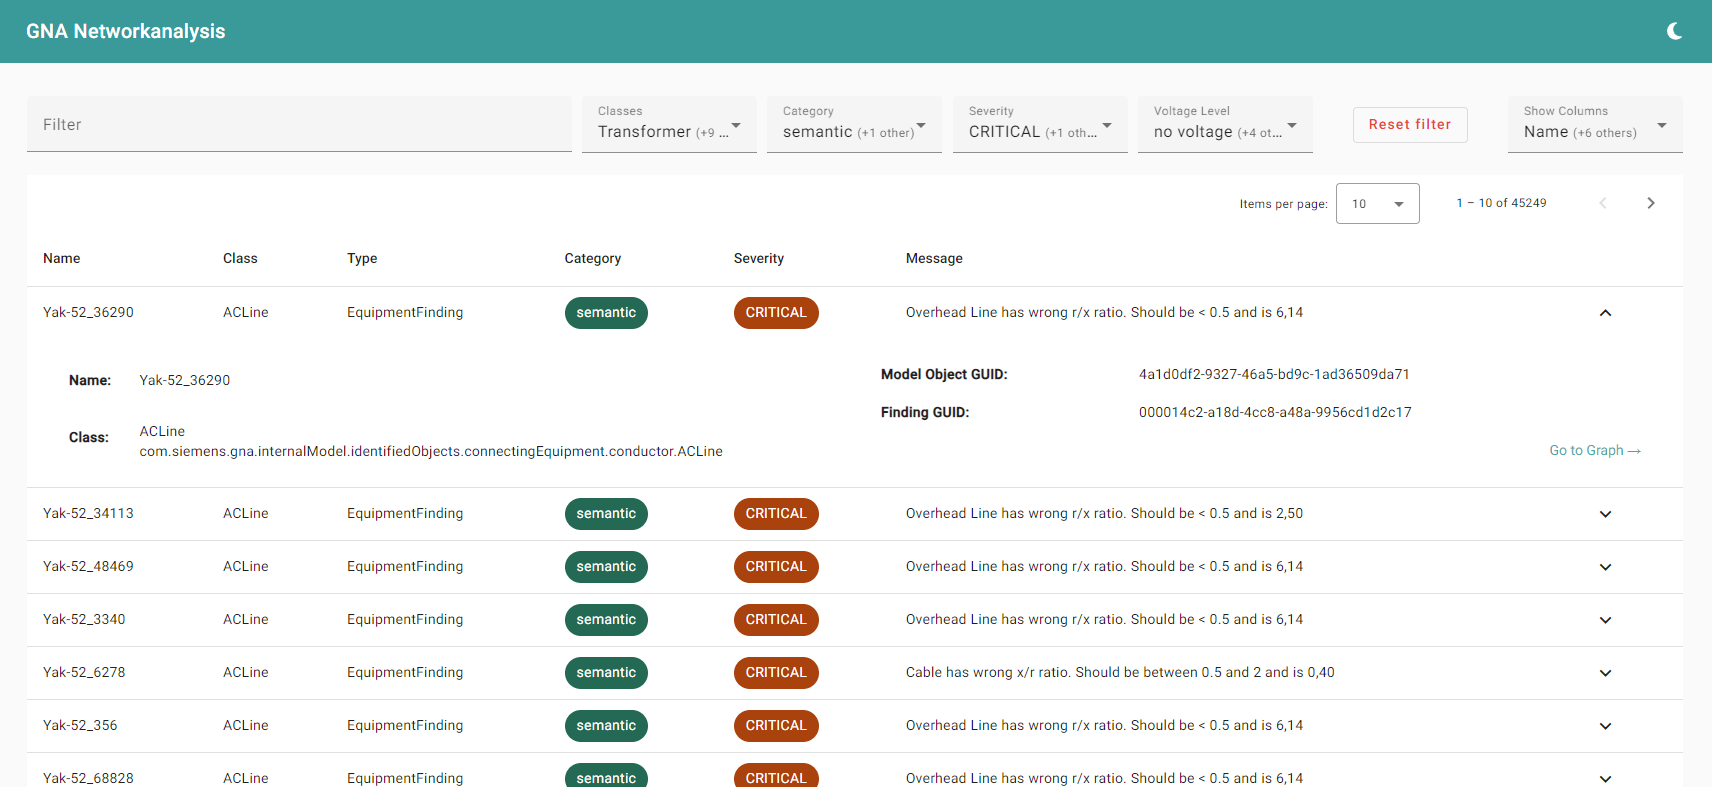
\includegraphics[width=1\textwidth]{content/img/Empire/Frontend/Angular_Findings_Prototype.png}
    \caption{Tabelle mit den aktuellen Fehlern im Stromnetzwerk}
    \label{fig:AngularFindingsPrototype}
\end{figure}
\FloatBarrier

\subsection{Sortierung}

Ein wichtiger Bestandteil moderner Tabellen in der digitalen Welt ist die Möglichkeit einer Sortierung. Diese Implementation ist dank der Bibliothek, welche in unserem Prototypen für alle UI-Elemente verwendet wird, Angular Material wirklich einfach. Nach Einstellung der Art der Sortierung -- Diese kann variieren. Beispielsweise werden bei numerischer Sortierung Zahlen logisch der Größe nach geordnet, während alphabetisches Sortieren bei Zahlen keinen Sinn ergibt, da somit \wordindoublequotes{111} vor \wordindoublequotes{22} kommen würde. -- und richtiger Handhabung der Aktualisierung der Daten, sobald eine neue Spalte ausgewählt wird, funktioniert diese wirklich verlässlich. Diese Art der Implementierung ist auch als \wordindoublequotes{deklarative Programmierung} bekannt, da man dem Framework nur sagt, \emph{was} zu tun ist. Im Gegensatz zur 
 \wordindoublequotes{imperativen Programmierung} müssen nicht die einzelnen Schritte selbst implementiert werden -- \emph{wie} etwas zu tun ist.

 In Abbildung \ref{fig:AngularFindingsSortingTypePrototype} können Sie sehen, dass die Datensätze alphabetisch aufsteigend nach dem Typen geordnet sind, wie auch an dem kleinen Pfeil neben dem Spaltennamen erkennbar ist.

\begin{figure}
    \centering
    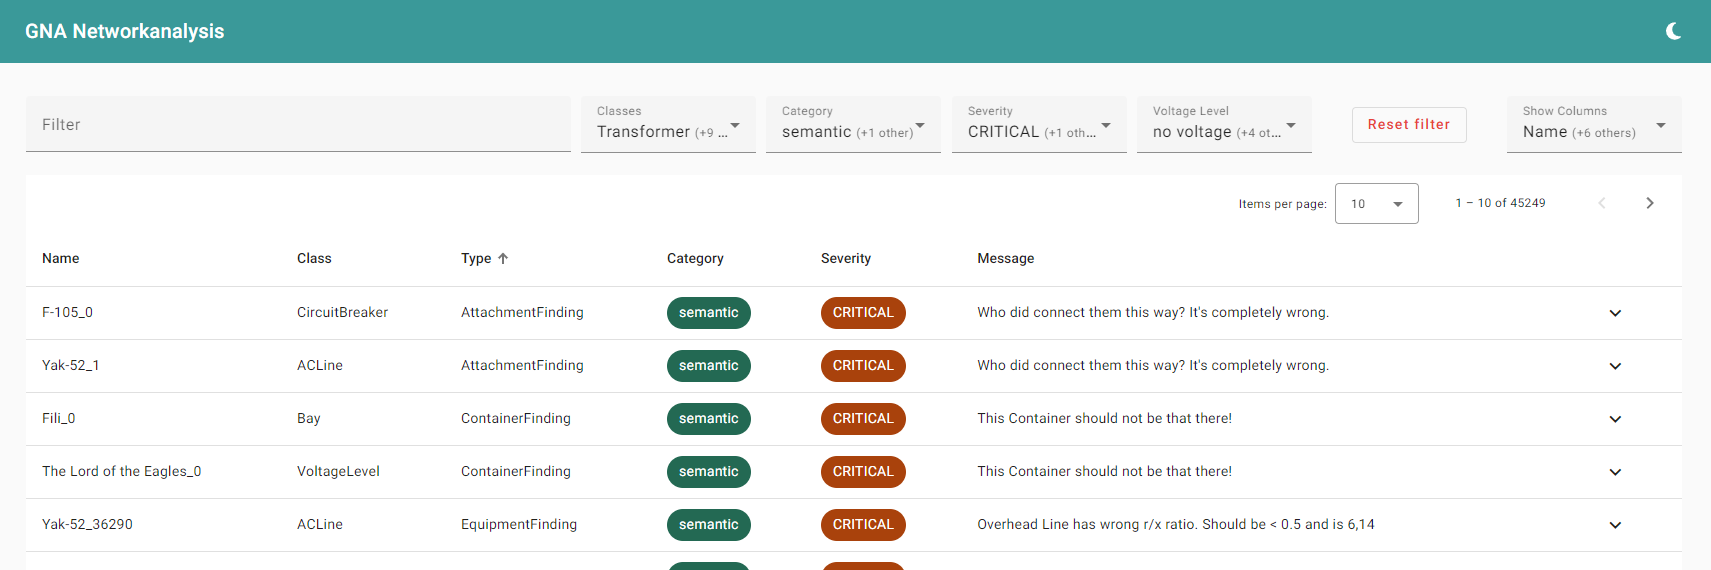
\includegraphics[width=1\textwidth]{content/img/Empire/Frontend/Angular_Findings_Sorting_Type_Prototype.png}
    \caption{Sortierungsoptionen der Tabelle des Prototypen}
    \label{fig:AngularFindingsSortingTypePrototype}
\end{figure}
\FloatBarrier

\subsection{Filterung}

Unsere Webapplikation verfügt außerdem über einige Filteroptionen. Dazu gehört natürlich ein Eingabefeld, welches über alle Spalten der Tabelle sucht und anschließend nur relevante Ergebnisse anzeigt. In Abbildung \ref{fig:AngularFindingsFilteringNodePrototype} sehen Sie beispielsweise die Filterung nach dem Wort \wordindoublequotes{Node}, welches bei den ersten drei Ergebnissen in der Klasse und ansonsten auch immer in der Nachricht des Eintrages vorkommt. Dieses Eingabefeld ist laut Siemens auch besonders wichtig, um schnell nach bestimmten Fehlern mit einer konkreten ID suchen zu können. Hierbei können Sie diese Identifikatoren zwar nicht als eigene Spalte sehen, jedoch sind sowohl die GUID des Fehlers als auch die GUID des Objektes, wo dieser Fehler im Stromnetzwerk auftritt, unter den zusätzlichen Informationen sichtbar. In Abbildung \ref{fig:AngularFindingsPrototype} haben Sie bereits diese Zusatzinformationen einsehen können.

\begin{figure}
    \centering
    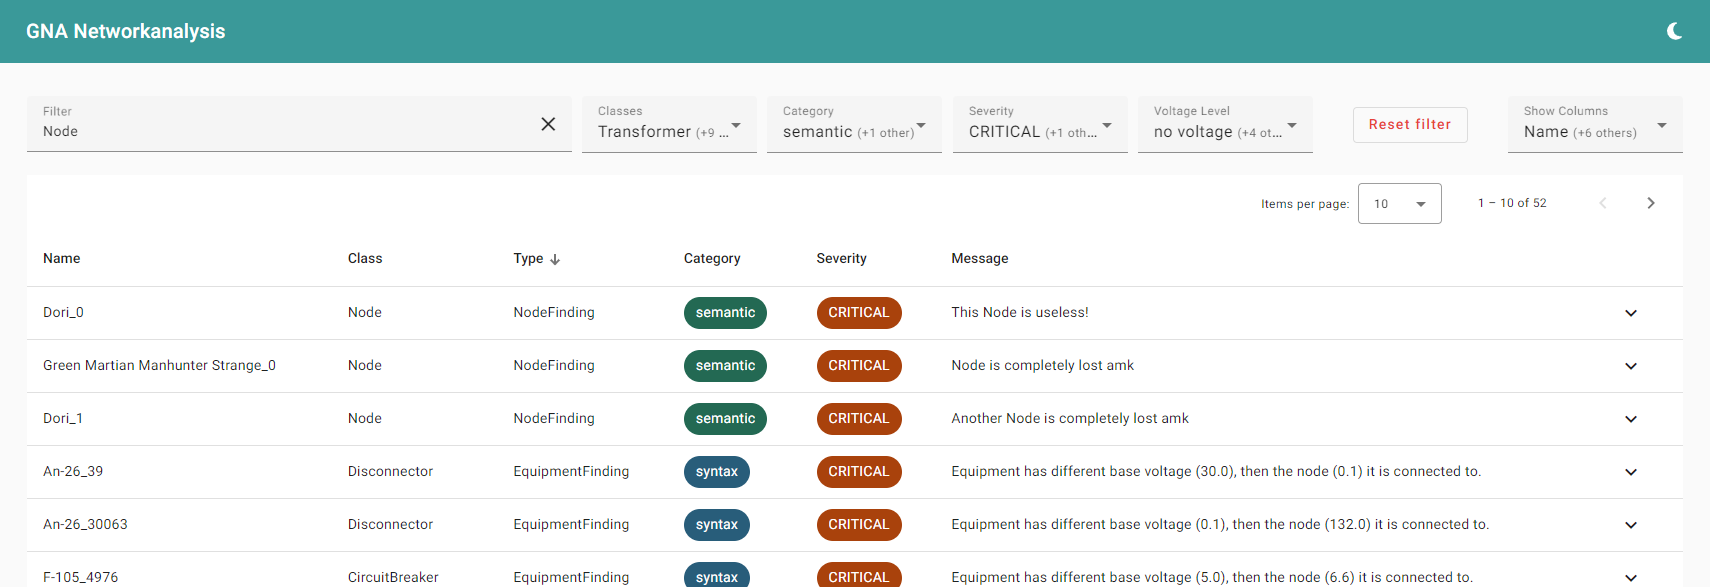
\includegraphics[width=1\textwidth]{content/img/Empire/Frontend/Angular_Findings_Filtering_Node_Prototype.png}
    \caption{Filterungsoption mit Eingabefeld über alle Spalten}
    \label{fig:AngularFindingsFilteringNodePrototype}
\end{figure}
\FloatBarrier

Im Laufe des Projektes ist noch die Anforderung hinzugekommen, die Einschränkung der Daten nach bestimmten Kriterien filter zu können. Hierbei handelt es sich genau wie beim Dashboard \ref{chp:dashboard} um die vier Eigenschaften: Klasse, Kategorie, Schweregrad und Spannungslevel. Im untigen Beispiel \ref{fig:AngularFindingsFilteringSeverityPrototype} ist die Einschränkung der Netzwerkfehler des Schweregrads abgebildet.

\begin{figure}
    \centering
    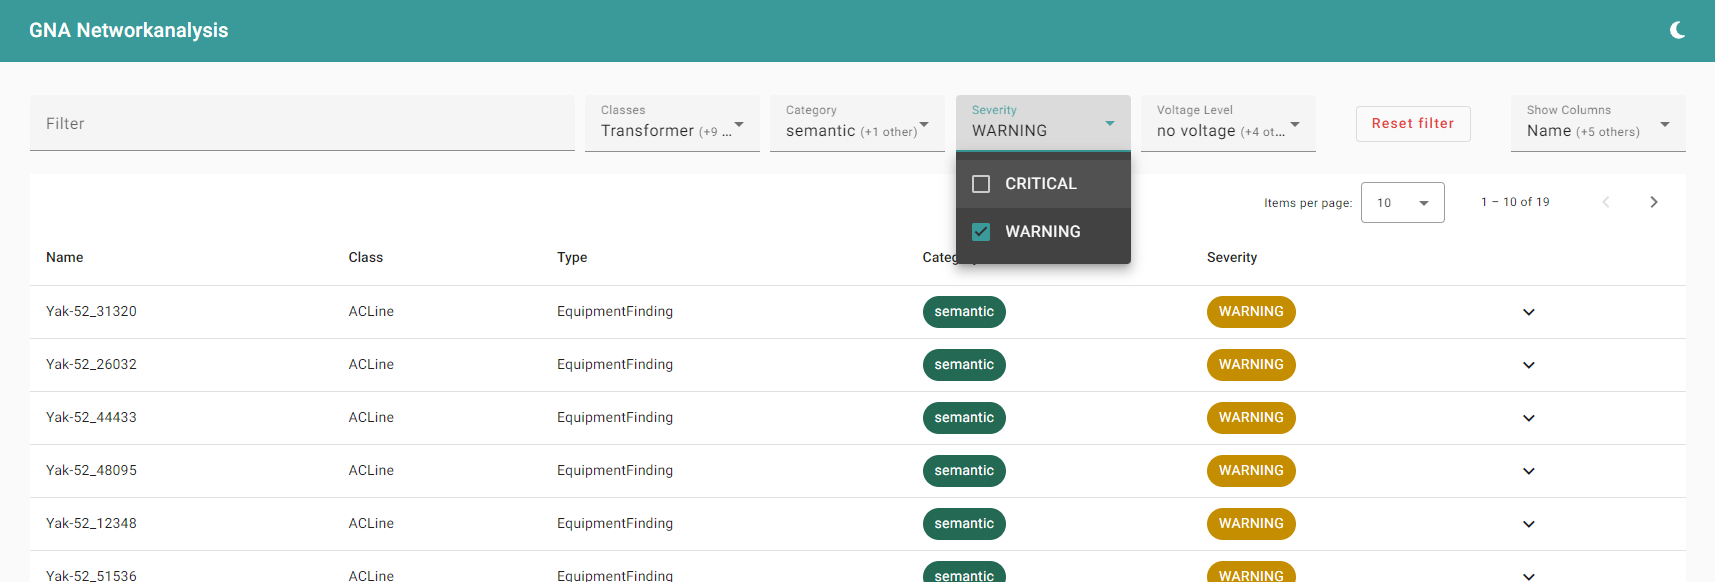
\includegraphics[width=1\textwidth]{content/img/Empire/Frontend/Angular_Findings_Filtering_Severity_Prototype.png}
    \caption{Filterungsmöglichkeit mit Dropdown-Menu für Schweregrad}
    \label{fig:AngularFindingsFilteringSeverityPrototype}
\end{figure}
\FloatBarrier

Eine wichtige Komponente der Filterungsmöglichkeiten ist der Reset-Button. Dieser erlaubt das schnelle Zurücksetzen aller Filter, falls der Benutzer das Gefühlt hat, sich in den Tiefen der Filterungsoptionen verirrt zu haben. Trotz seiner Einfachheit hat der Reset-Button in vielen Fällen eine hohe Daseinsberechtigung, da er intuitiv und äußerst nützlich ist.

\subsection{Paginierung}

Im Stromnetzwerk treten stetig einige Fehler auf, da das Netzmodell konstant umgebaut und verbessert wird. Eine \emph{GraphQL}-Abfrage, welche all diese Daten auf einmal anzeigen wollen würde, führe zwangsmäßig zu langen Ladezeiten. Aus diesem Grund hat heutzutage jeder Anwendungsfall, welcher mit vielen Daten arbeitet, irgendeine Art Pagination eingebaut. Dabei wird einfach nur ein bestimmter Teil der Daten geladen. Andere Datensätze können nach Bedarf nachgeladen werden. Während viele Social Media-Platformen auf Lazy Loading setzen -- hierbei werden neue Daten beim Scrollen nachgeladen -- verwendet unsere Applikation die von Angular Material ausimplementierte Pagination. Der Nutzer kann hierbei einfach auf die beiden Pfeile rechts oben klicken, um weitere Einträge zu laden. Um die Orientierung über die Daten zu behalten, werden außerdem ständig Informationen bezüglich den momentan angezeigten Elementen dargestellt. Beispielsweise lässt sich der Nutzer in Abbildung \ref{fig:AngularFindingsPaginationPrototype} gerade die Elemente 351 bis 375 anzeigen. Insgesamt verfügen unsere Testdaten über 45.249 Datensätze.

\begin{figure}
    \centering
    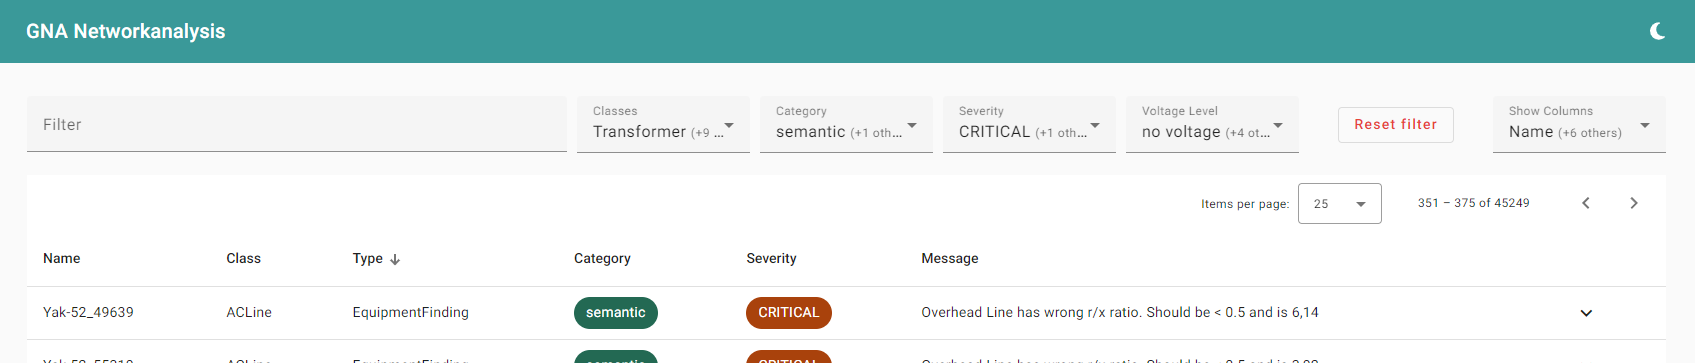
\includegraphics[width=1\textwidth]{content/img/Empire/Frontend/Angular_Findings_Pagination_Prototype.png}
    \caption{Paginierung der Tabelle mit den Fehlern}
    \label{fig:AngularFindingsPaginationPrototype}
\end{figure}
\FloatBarrier

\subsection{Besonderheit: Spannung}

Einige Datensätze verfügen über die zusätzliche Information des Spannungslevels. Dieses wird dynamisch unter den zusätzlichen Informationen angezeigt und außerdem können Sie nach diesen Werten filtern, da sie eine große Bedeutung im Stromnetzwerk haben. Aufgrund von Zeitmangel ist sich die Implementation der rekursiven Abfragen nach dem Spannungslevel nicht mehr ausgegangen. Das Netzmodell ist nämlich vereinfacht geschrieben in einer Baumstruktur aufgebaut. Teilweise haben Container höher in dieser Struktur Informationen bezüglich der Spannung des gesamten Bereiches. Jedoch hätte bei der Implementierung dieser Funktionalität die Rekursion zur Auflösung des Baummodells eine komplexere Datenabfrage zur Folge gehabt, weshalb auf dieses Feature verzichtet worden ist. Dieses Leistungsmerkmal könnte zukünftig noch erweitert werden.

Der anonymisierte Eintrag \wordindoublequotes{Giant Cyclops X\_24} in Abbildung \ref{fig:AngularFindingsVoltagePrototype} verfügt zum Beispiel über ein Spannungslevel von 220kV.

\begin{figure}
    \centering
    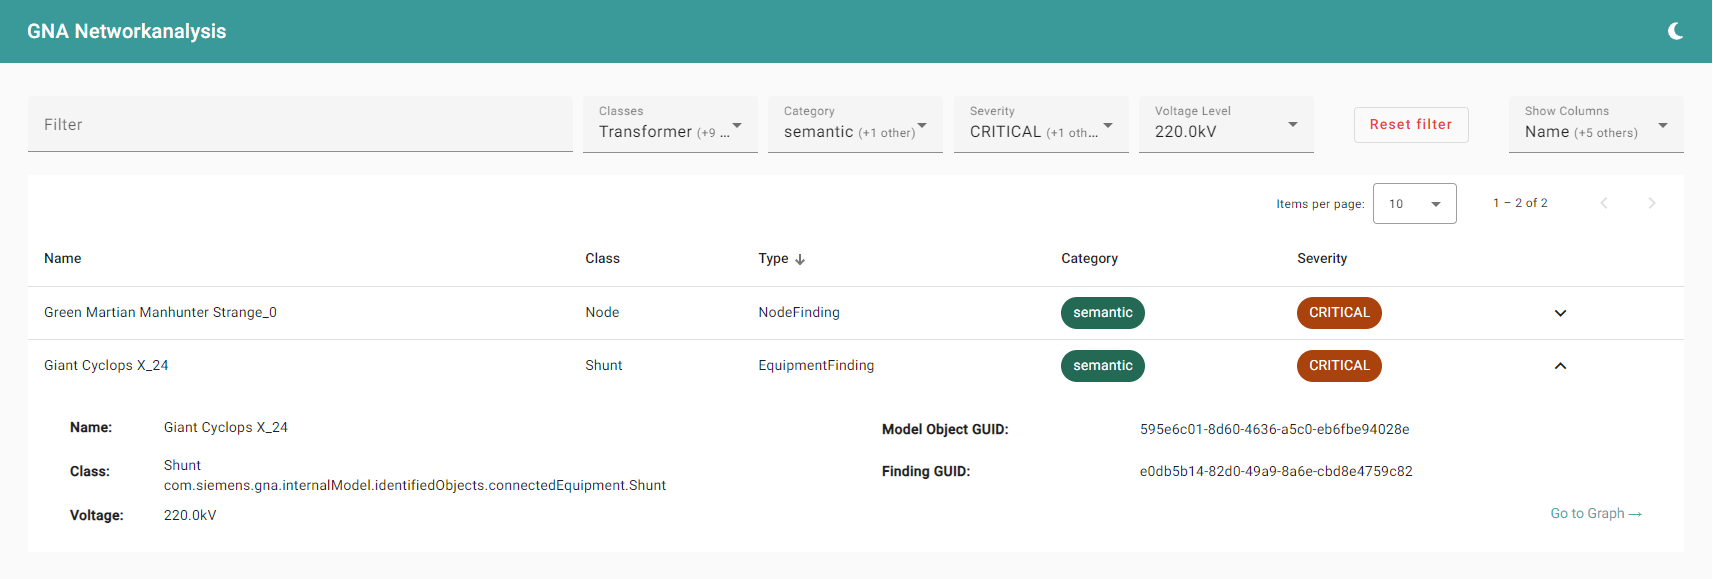
\includegraphics[width=1\textwidth]{content/img/Empire/Frontend/Angular_Findings_Voltage_Prototype.png}
    \caption{Einträge, welche über einen Spannungswert von 220.0kV verfügen}
    \label{fig:AngularFindingsVoltagePrototype}
\end{figure}
\FloatBarrier

Wie Sie in dieser Abbildung (\ref{fig:AngularFindingsVoltagePrototype}) auch schön sehen können, verfügt jeder Eintrag über einen \wordindoublequotes{Go to Graph →}-Button unten rechts. Wohin dieser den Benutzer führt, wollen wir uns als nächstes ansehen.